\documentclass[../th_cyber_warfare_distilled.tex]{subfiles}
 
\begin{document}
\chapter{ภัยคุกคามไซเบอร์}

ความก้าวหน้าของเทคโนโลยีสารสนเทศและการสื่อสารส่งผลโดยตรงต่อแนวคิดเกี่ยวข้องกับการปฏิบัติการทางทหาร โดยเห็นได้จากการประยุกต์ใช้โครงสร้างพื้นฐานเทคโนโลยีสารสนเทศและระบบเครือข่ายในการปฏิบัติภารกิจเพื่อความมั่นคงในหลากหลายมิติ เช่น ระบบควบคุมบังคับบัญชา ระบบค้นหา วิเคราะห์ และประเมินค่าเป้าหมาย ด้วยเหตุที่ว่าเทคโนโลยีสารสนเทศและการสื่อสารช่วยให้วงรอบการตัดสินใจของผู้บังคับบัญชารวดเร็วและตอบสนองต่อสถานการณ์ที่เปลี่ยนแปลงไปได้อย่างแม่นยำ จนกล่าวได้ว่าการประยุกต์ใช้เทคโนโลยีสารสนเทศและการสื่อสารได้อย่างเหมาะสมจะเพิ่มโอกาสที่หน่วยจะบรรลุภารกิจ 

เครือข่ายอินเทอร์เน็ตซึ่งในระยะเริ่มแรกถูกพัฒนาขึ้นเพื่อตอบโจทย์เกี่ยวกับสงครามนิวเคลียร์ โดยถูกออกแบบให้มีความพร้อมใช้ มีความเข้ากันได้กับอุปกรณ์แตกต่างชนิด และสามารถทำงานได้แม้ว่าเครือข่ายส่วนหนึ่งจะถูกทำลายไปจากอาวุธนิวเคลียร์ โดยในระหว่างยุคแรกๆของการพัฒนาไม่ได้มีการพิจารณาปัจจัยเกี่ยวกับความมั่นคงปลอดภัยจนเมื่อเกิดการแพร่ระบาดของหนอนอินเทอร์เน็ต (worm) ใน ค.ศ.1980 จึงมีความตระหนักรู้ถึงความเสี่ยงด้านความมั่นคงปลอดภัยของเครือข่ายอินเทอร์เน็ตเป็นครั้งแรก และมีรายงานความมั่นคงปลอดภัยของเครือข่ายอินเทอร์เน็ตอย่างต่อเนื่องจนถึงปัจจุบัน

\section{กำลังอำนาจแห่งชาติ}
การประเมินกำลังอำนาจแห่งชาติสามารถกระทำได้หลากหลายไม่ว่าจะเป็น DIME -- Diplomatic, Information, Military, Economy หรือ MIDLIFE -- Military, Intelligence, Diplomatic, Law Enforcement, Information, Finance, Economic หรือ PMESII -- Political, Military, Economic, Social, Informational, Infrastructure โดยเมื่อพิจารณาอย่างถี่ถ้วนจะพบว่าองค์ประกอบของกำลังอำนาจแห่งชาติที่ได้ยกตัวอย่างมีความเหลื่อมทับระหว่างกันโดยเฉพาะอย่างยิ่งข้อมูลข่าวสารซึ่งปรากฎอยู่ในทุกๆแนวคิด เนื่องจากข้อมูลข่าวสารเป็นปัจจัยอันดับต้นๆที่ต้องคำนึงถึงในการทำสงครามทุกๆสมรภูมิ ประกอบกับความก้าวหน้าของเทคโนโลยีสารสนเทศและการสื่อสารที่มีความก้าวหน้าแบบก้าวกระโดดในช่วง 2-3 ทศวรรษที่ผ่านมาจึงทำให้การสร้าง ประมวลผล และแพร่กระจายข้อมูลข่าวสารกระทำได้อย่างรวดเร็ว ในที่นี้ผู้เขียนจะใช้ DIME ในการเปรียบเทียบและวิเคราะห์เนื่องจาก DIME ยังคงถูกใช้งานอย่างแพร่หลายในหลักนิยมของกองทัพสหรัฐซึ่งเป็นหลักนิยมหลักที่กองทัพไทยนำมาประยุกต์ใช้

\section{ภัยคุกคามทางไซเบอร์}

การโจมตีต่อโครงสร้างพื้นฐานระบบสารสนเทศและการสื่อสารถูกรายงานเป็นครั้งแรกในช่วงทศวรรษที่ 1990 โดยมีเหตุการณ์สำคัญๆ เช่น ในปี 1999 กระทรวงกลาโหมสหรัฐอเมริการายงานการถูกโจมตีจากระบบเครือข่ายที่มีต้นทางจากสหภาพโซเวียตและส่งผลให้ข้อมูลสำคัญเกี่ยวกับเทคโนโลยีทางทหารถูกโจรกรรม และเชื่อกันว่าเป็นเหตุการณ์ความมั่นคงปลอดภัยทางเครือข่ายที่มีรัฐเป็นตัวแสดงครั้งแรก  อย่างไรก็ตามสหภาพโซเวียตปฏิเสธความรับผิดชอบโดยสิ้นเชิงต่อเหตุการณ์ดังกล่าว โดยเหตุการณ์ในครั้งนั้นได้รับชื่อว่า ``Moonlight Maze" ต่อมาในปี  2007 กลุ่มแฮกเกอร์ที่เชื่อกันว่าได้รับการสนับสนุนจากรัฐบาลรัสเซียทำการโจมตีต่อเว็บไซต์ของหน่วยงานราชการเอสโตเนียจนรัฐบาลเอสโตเนียต้องขอรับการสนับสนุนทรัพยากรจากประเทศในกลุ่ม NATO เข้ามาช่วยแก้ปัญหาและฟื้นคืนระบบ และปรากฎรายงานเหตุการณ์ความมั่นคงปลอดภัยเกิดขึ้นอย่างต่อเนื่องจนถึงปัจจุบัน

ในปัจจุบันหน่วยงานในรัฐบาลสหรัฐอเมริกานิยมเรียกเหตุการณ์ด้านความมั่นคงปลอดภัยที่มี ``รัฐ" เป็นตัวแสดงว่า ``Advance Persistent Threat: APT" โดยผลกระทบที่เกิดขึ้นจะส่งผลต่อความมั่นคงปลอดภัยของโครงสร้างพื้นฐานข้อมูลข่าวสารของรัฐที่ถูกโจมตีโดยขอบเขตความมั่นคงปลอดภัยจะครอบคลุมถึง การรักษาความลับ การรักษาความครบถ้วนสมบูรณ์ และการรักษาความพร้อมใช้ ของทรัพยากรสารสนเทศและการสื่อสารซึ่งเป็นองค์ประกอบหนึ่งของกำลังอำนาจแห่งชาติ (DIME)



\paragraph{ภัยคุกคาม (Threats)}
หมายถึง บุคคล เหตุการณ์ ใดๆก็ตามที่เป็นสาเหตุของการลดทอดความมั่นคงปลอดภัยของทรัพยากรสารสนเทศซึ่งประกอบด้วยโครงสร้างพื้นฐานระบบสารสนเทศและการสื่อสาร ตลอดจนข้อมูลข่าวสารที่รับ-ส่งผ่านช่องทางการสื่อสาร โดยภัยคุกคามดังกล่าวรวมไปถึงเหตุการณ์ที่เกิดขึ้นโดยภัยธรรมชาติและอุบัติเหตุ โดยบุคคลที่ทำการโจมตีนิยมเรียกกว่า ``ผู้ไม่ประสงค์ดี" ``ผู้บุกรุก"  หรือ ``แฮกเกอร์" เมื่อพิจารณาถึงแหล่งที่มาของการโจมตีจะสามารถจำแนกแหล่งที่มาได้ 2 ลักษณะ ได้แก่
\begin{itemize}
	\item \textbf{ผู้บุกรุกจากภายนอก} หมายถึง ผู้บุกรุกที่ทำการโจมตีต่อทรัพยากรสารสนเทศจากภายนอกองค์กร
	\item \textbf{ผู้บุกรุกจากภายใน} หมายถึง ผู้บุกรุกที่ทำการโจมตีต่อทรัพยากรสารสนเทศจากภายในองค์กร
\end{itemize}
\par
ทั้งนี้ผู้ไม่ประสงค์ดีอาจมีแรงจูงใจในการโจมตีต่อทรัพยากรสารสนเทศและการสื่อสารที่แตกต่างกันออกไปเช่น ความเชื่อพื้นฐานทางศาสนา ลัทธิการเมือง แรงจูงใจทางการเงิน ชื่อเสียง ความอยากรู้อยากเห็น ฯลฯ


\section{ผลกระทบของภัยคุกคามทางไซเบอร์}

%\begin{minipge}{12cm}
\paragraph{ผลกระทบของการโจมตี}
\begin{figure}
	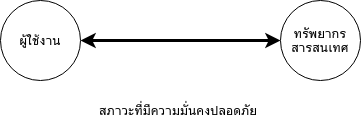
\includegraphics[scale=0.35]{figure_secured_usage.png}
	\centering
	\caption{สภาวะที่มีความมั่นคงปลอดภัย}
	\label{figure:secured_usage}
\end{figure}

\begin{figure}
	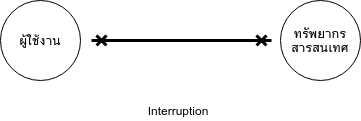
\includegraphics[scale=0.35]{insecure_interruption.png}
	\centering
	\caption{การสกัดขัดขวาง}
	\label{figure:insecure_interruption}
\end{figure}

\begin{figure}
	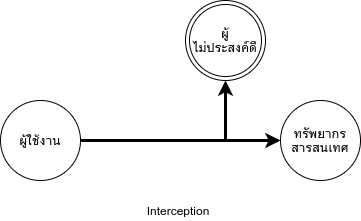
\includegraphics[scale=0.35]{insecure_interception.png}
	\centering
	\caption{การดักรับดักฟัง}
	\label{figure:insecure_interception}
\end{figure}

\begin{figure}
	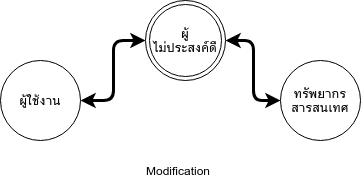
\includegraphics[scale=0.35]{insecure_modification.png}
	\centering
	\caption{การเปลี่ยนแปลงแก้ไข}
	\label{figure:insecure_modification}
\end{figure}

\begin{figure}
	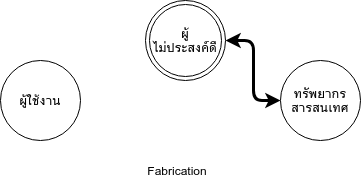
\includegraphics[scale=0.35]{insecure_fabrication.png}
	\centering
	\caption{การปลอมแปลง}
	\label{figure:insecure_fabrication}
\end{figure}

การเข้าถึงและใช้ประโยชน์จากทรัพยาการสารสนเทศและการสื่อสารของผู้ใช้งานหากเป็นไปอย่างมั่นคงปลอดภัยสามารถแสดงได้ดังภาพที่ \ref{figure:secured_usage} โดยจะเห็นว่าผู้ใช้งานจะสามารถเข้าใช้งานทรัพยากรสารสนเทศได้โดยไม่มีบุคคลอื่นเข้าถึงทรัพยากรที่ผู้ใช้งานเข้าถึงอยู่โดยไม่มีสิทธิ์ ทั้งนี้เมื่อจำแนกผลกระทบของการโจมตีต่อทรัพยากรสารสนเทศไม่ว่าจะมีแหล่งกำเนิดจากภายในหรือภายนอกองค์กรจะสามารถจำแนกได้ 4 ประเภท ได้แก่




\begin{enumerate}
	\item \textbf{การสกัดขัดขวาง (Interruption)} คือ การทำให้ทรัพยากรสารสนเทศไม่สามารถให้บริการได้ เช่น การเข้ารหัสไฟล์หรือฮาร์ดดิสก์โดยซอฟต์แวร์เรียกค่าไถ่ การโจมตีแบบกระจาย (Distributed Denial of Service: DDoS) การขโมยอุปกรณ์ ดังแสดงในภาพที่ \ref{figure:insecure_interruption} ยกตัวอย่างการขโมยอุปกรณ์ย่อมส่งผลให้ผู้ใช้งานไม่สามารถเข้าถึงทรัพยากรนั้นๆได้ 
	


	\item \textbf{การดักรับดักฟัง (Interception)} คือ การเข้าถึงทรัพยากรสารสนเทศระหว่างที่กำลังถูกส่งผ่านระบบการสื่อสารหรือระบบเครือข่าย เช่น การใช้โปรแกรม sniffer ดักรับดักฟังเครือข่าย หรือการดักรับสัญญาณที่แพร่กระจาย การคุ้ยขยะเพื่อค้นหาข้อมูลสำหรับเข้าใช้งานระบบ ดังแสดงในภาพที่ \ref{figure:insecure_interception} จะเห็นว่าทรัพยากรสารสนเทศเหล่านั้นจะถูกเข้าถึงได้จากผู้ไม่ประสงค์ดีซึ่งถ้าหากปราศจากมาตรการป้องกันที่เหมาะสมผู้ไม่ประสงค์ดีย่อมทำความเข้าใจและล่วงรู้ถึงข้อมูลที่รับ-ส่งนั้นๆได้ 

	\item \textbf{การเปลี่ยนแปลงแก้ไข (Modification)} คือ การทำให้ทรัพยากรสารสนเทศและการสื่อสารถูกเปลี่ยนสภาพไปโดยไม่มีสิทธิ์ หรือไม่ได้รับอนุญาต ดังแสดงในภาพที่ \ref{figure:insecure_modification} ในที่นี้จะยกตัวอย่าง การเปลี่ยนแปลงแก้ไขข้อมูลเงินเดือนในระบบงานเงินเดือน การแก้ไขหน้าเว็บโดยไม่ได้รับอนุญาต  



	\item \textbf{การปลอมแปลง (Fabrication)} คือ การสร้างทรัพยากรสารสนเทศและการสื่อสารเข้าสู่โครงสร้างพื้นฐานหรือระบบ เช่นการปลอมข้อมูล หรือการปลอมแปลงตัวตน ดังแสดงในภาพที่ \ref{figure:insecure_fabrication}

\end{enumerate}

เมื่อพิจารณาผลกระทบของการโจมตีต่อทรัพยากรสารสนเทศและการสื่อสารดังที่ได้กล่าวมาจะมีความเชื่อมโยงกับหลักการรักษาความมั่นคงปลอดภัยระบบสารสนเทศและการสื่อสารซึ่งประกอบด้วย การรักษาความลับ (Confidentiality) การรักษาความครบถ้วนสมบูรณ์ (Integrity) และการรักษาความพร้อมใช้ (Avalibility) ของทรัพยากรสารสนเทศและการสื่อสารทั้งปวง โดยจะได้กล่าวถึงหลักการรักษาความมั่นคงปลอดภัยโดยละเอียดต่อไปในบทที่ \ref{chapter:cyberwar_doctrine}

%\end{minipage}

\section{ประเภทของภัยคุกคาม}
\paragraph{การจำแนกประเภทภัยคุกคาม}
เมื่อพิจารณาผลกระทบของภัยคุกคามที่ได้กล่าวมาแล้วจะพบว่าแนวทางการโจมตีต่อทรัพยากรสารสนเทศและการสื่อสารจะถูกแบ่งเป็น 2 ลักษณะคือ ภัยคุกคามแบบแอคทีฟ (active threats) และภัยคุกคามแบบพาสซีฟ (passive threats)
\begin{itemize}
	\item \textbf{ภัยคุกคามแบบแอคทีฟ} หมายถึง การโจมตีที่ผู้ไม่ประสงค์ดีอาจถูกตรวจพบได้จากกระบวนการเฝ้าตตรวจความมั่นคงปลอดภัย เช่นการทำให้ระบบปฏิเสธการให้บริการด้วยมัลแวร์จำพวกบอทเน็ต (DDoS via botnet) SQL Injection การโจมตีแบบคนกลาง (Man-In-The-Middle) เป็นต้น
	\item \textbf{ภัยคุกคามแบบพาสซีฟ} หมายถึง การโจมตีที่ผู้ไม่ประสงค์ดีจะไม่ถูกตรวจพบจากกระบวนการการเฝ้าตรวจความมั่นคงปลอดภัย เช่นการดักรับดักฟัง (eavesdropping and sniffing) การสืบค้นข้อมูลจาก search engine การโจมตีด้วยเทคนิควิศวกรรมเชิงสังคม (social engineering) เป็นต้น 
\end{itemize}

\paragraph{ภัยคุกคามจำแนกจากแรงจูงใจ}

แรงจูงใจที่ทำให้ผู้ไม่ประสงค์ดีตัดสินใจโจมตีต่อโครงสร้างพื้นฐานเทคโนโลยีสารสนเทศและการสื่อสารแตกต่างกันในแต่ละบุคคลและกลุ่มบุคคล และด้วยแรงจูงใจที่แตกต่างกันย่อมส่งผลต่อผลกระทบต่อพลังอำนาจแห่งชาติในระดับที่แตกต่างกันออกไปดังแสดงในภาพที่ \ref{figure:cyber_incident} แสดงเหตุการณ์การโจมตีทางไซเบอร์ต่อโครงสร้างพื้นฐานระบบสารสนเทศและการสื่อสารของประเทศต่างๆหลายประเทศ เมื่อรวบรวมหลักฐานจากเหตุการณ์ที่ผ่านๆมาจะสามารถจำแนกแรงจูงใจเหล่านั้นได้หลายประการดังนี้


\begin{figure}
	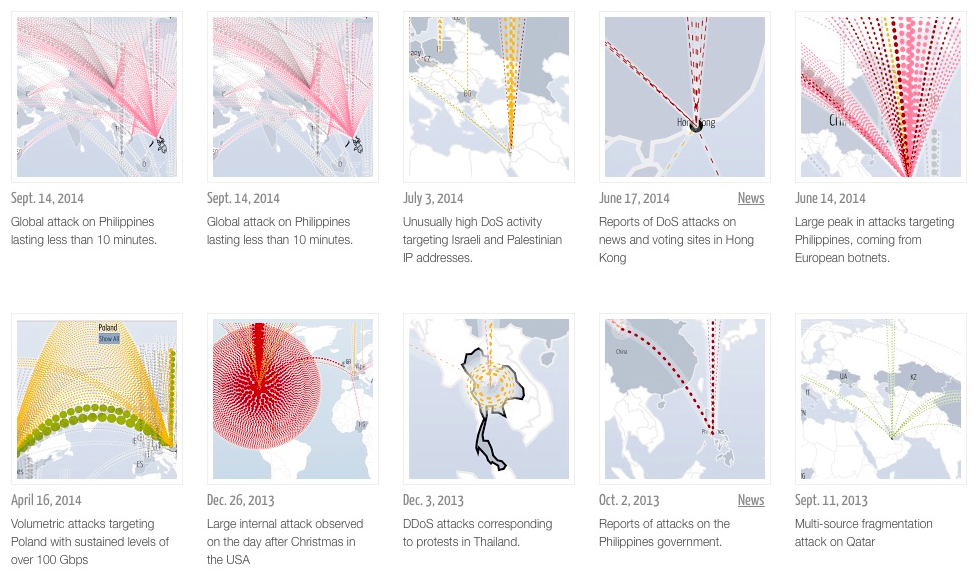
\includegraphics[scale=0.35]{image_warzone.png}
	\centering
	\caption{ภัยคุกคามทางไซเบอร์ขนาดใหญ่}
	\label{figure:cyber_incident}
\end{figure}


\begin{itemize}
	\item \textbf{Script Kiddy} หมายถึง ภัยคุกคามทางไซเบอร์ที่เกิดจากผู้ที่ชอบศึกษาทดลองซอฟต์แวร์สำหรับเจาะระบบ แต่ไม่มีความสามารถในการพัฒนาซอฟต์แวร์จึงต้องใช้ซอฟต์แวร์ที่ถูกพัฒนาขึ้นมาจากแฮกเกอร์ที่มีความสามารถสูงโดยซอฟต์แวร์เหล่านั้นสามารถดาว์นโหลดได้จากแหล่งซอฟต์แวร์เปิดบนเครือข่ายอินเทอร์เน็ต โดยพบว่าเหตุการณ์ด้านความมั่นคงปลอดภัยส่วนใหญ่เป็นผลจากการโจมตีกลุ่มคนในกลุ่มนี้และพบว่าผลเสียหายที่เกิดขึ้นไม่มีนัยสำคัญอย่างไรต่อพลังอำนาจแห่งชาติ
	\item \textbf{Criminal} หมายถึง ภัยคุกคามทางไซเบอร์ที่เกิดขึ้นจากแรงขับเคลื่อนขององค์กรอาชญากรรมที่มุ่งหาประโยชน์จากการโจมตีโครงสร้างพื้นฐานเทคโนโลยีสารสนเทศและการสื่อสาร จากสถิติพบกว่าปริมาณการโจมตีที่เกิดขึ้นจากกลุ่มนี้มีจำนวนมากรองลงมาจากการโจมตีของกลุ่มสคริปคิดดี้ 
	\item \textbf{Hacker Groups} หมายถึง ภัยคุกคามทางไซเบอร์ที่เป็นผลของการดำเนินกิจกรรมของกลุ่มแฮกเกอร์ที่มีฝีมือโดยมักเป็นผู้พัฒนาเครื่องมือสำหรับใช้โจมตีต่อโครงสร้างพื้นฐานระบบสารสนเทศโดยพบว่าผลกระทบของภัยคุกคามจากกลุ่มนี้มีมากถึงร้อยละ 80 ของผลเสียหายทั้งหมด ลักษณะเฉพาะของภัยคุกคามจากกลุ่มนี้คือการกระทำเพื่อหวังผลประโยชน์ในรูปของตัวเงิน และเศรษฐกิจ
	\item \textbf{Insider} หมายถึง ภัยคุกคามทางไซเบอร์ที่เป็นผลการดำเนินการของกลุ่มคนภายในองค์กร ซึ่งเป็นจุดที่มักจะได้รับการปกป้องต่ำกว่าโครงสร้างพื้นฐานที่เชื่อมต่อกับเครือข่ายภายนอก โดยมีแรงจูงใจในการกระทำส่วนใหญ่เพื่อแก้แค้นองค์กร หรือได้รับการสนับสนุนทางการเงินจากองค์กรคู่แข่ง 
	\item \textbf{Political/Religious} หมายถึง ภัยคุกคามทางไซเบอร์ที่เป็นผลของการดำเนินการจากบุคคลที่มีความเชื่อทางการเมืองตรงข้ามกระทำต่อกันเพื่อล้มล้างหรือสร้างสภาวะที่ฝ่ายตนต้องการ โดยมักไม่หวังผลความเสียหายต่อพลังอำนาจแห่งชาติ อย่างไรก็ดีเมื่อพิจารณาขอบเขตการใช้ความเชื่อทางศาสนาเป็นเครื่องมือจะพบว่าแนวโน้มการใช้โครงสร้างพื้นฐานเทคโนโลยีสารสนเทศและการสื่อสารในการปลูกฝังและขยายจำนวนผู้ร่วมอุดมการณ์ของกลุ่มก่อการร้ายเพิ่มขึ้นอย่างมีนัยสำคัญ
	\item \textbf{APT/Nation/State} หมายถึง ภัยคุกคามทางไซเบอร์ที่มี ``รัฐ" เป็นผู้ดำเนินการหรือเป็นผู้ให้การสนับสนุน ดังนั้นการโจมตีที่เกิดขึ้นจึงอาจเกิดขึ้นจากกองกำลังตามแบบหรือกลุ่มแฮกเกอร์ที่ได้รับการสนับสนุนทั้งโดยตรงและทางอ้อม โดยปรากฎรายงานการจัดตั้งหน่วยงานสำหรับการปฏิบัติการไซเบอร์อย่างต่อเนื่อง เช่น The Tenth Fleet - The U.S. Fleet Cyber Command
\end{itemize}

สงครามไซเบอร์เป็นพื้นที่ยุทธภูมิใหม่ซึ่งเกิดขึ้นตามสภาพการเปลี่ยนแปลงทางยุทธศาสตร์ที่เป็นผลจากความก้าวหน้าของเทคโนโลยีสารสนเทศและการสื่อสาร อย่างไรก็ดีสิ่งที่ไม่เคยเปลี่ยนแปลงไปเลยคือการใช้กำลังอำนาจแห่งชาติเพื่อควบคุมพื้นที่สนามรบ (Battle Space) อันได้แก่ พื้นที่ทางบก พื้นที่ทางทะเล ห้วงอากาศ อวกาศ และไซเบอร์ ในบทต่อไปจะได้กล่าวถึงลักษณะเฉพาะและหลักนิยมของการปฏิบัติทางทหารในพื้นที่สนามรบแต่ละแบบ
\end{document}